\section{Inference}
\label{sec:soft-inference}
%
%
In this section the inference process is analyzed on the neural network model,
taking into account that the two applications share the same code. In fact, when
the model is loaded into the buffer, it is interpreted by the TensorFlow Lite
library, returning the training information of the model and in particular the
information regarding the input and output of the model.
For this case, where you are interested in the problem of object detection, the
size of the image is requested at the input and the number of color channels in
this case is constant and fixed at three.
Furthermore, the function reported in listing 4534243 is analyzed, which allows
to adapt the model input with the data, that is, the images coming from the
camera, taking into account to satisfy the neural model input and to adapt the
information for the tensor calculation if in floating point, or in 8-bit
integers.
It also takes into account the process of quantization that took place during
the transformation from original model to lite model, in fact the input will
also be recalculated. 
For fully integer models, the inputs are unsigned integer 8-bit.\\ 
The mean and standard deviation (\texttt{std\_dev}), calculated as in
\eqref{eq:stddev}, values specify how to \texttt{uint8} values map to the float
input values used while training the model.
The mean is the integer value from $0$ to $255$ that maps to floating point
\texttt{$0.0\text{f}$}. 
\begin{equation}
\label{eq:stddev}
\text{\texttt{std\_dev}} = \frac{255}{\text{\texttt{float}}_\text{max}-\text{\texttt{float}}_\text{min}}
\end{equation}
%
%
\subsection{Architecture x86\_64}
\label{ssec:x86-bench-inference}
We analyze in particular the inference cycle following the reception of the
frame by the TCP socket described previously in section
(\ref{ssec:software-coral-analysis}). It can be seen in figure
(\ref{subfig:all-bench}) that the captured process, where it is possible to
identify the functions performed:
\begin{itemize}
	\item The dark green rectangle represents the socket's reception function.
	\item The lighter green rectangle, on the other hand, is the time needed to calculate the inference.
	\item The pink rectangle represents the time to update the image in the user interface.
\end{itemize}
Although only one thread is shown here, in the solution adopted the TensorFLow
Lite module uses 8 cores, but it is possible to set a number of cores greater
than or equal to 1.
Comparing the two figures (\ref{subfig:time-cycle}) and
(\ref{subfig:time-inference}) it is observed that the duration of the cycle is
approximately $64.376 \,\si{\milli\second}$ and the other hand the infercence time
is $54.251 \,\si{\milli\second}$.
This time includes the execution of the functions described above, from this it
is possible to deduce that the most onerous task in terms of time and the
reconstruction of the image by the socket inside the
\textbf{TcpClient::imageAvailable} function. 
Meanwhile, \textbf{ModelTesnorFLowLite::run}'s function starts after about $10
\,\si{\milli\second}$ to end almost simultaneously with the function. Then the
cycle repeats itself.
Performing the inference with the TensorFlow Lite model, described in section
(\ref{sec:soft-inference}), on a laptop equipped with an Intel i7-7820HQ CPU
$2.90 \,\si{\giga\hertz}$ processor shows the benefits due to compression and
quantization of the neural model.
In particular, it is observed that the average time is $78 \,\si{\milli\second}$
therefore a considerable performance boost if compared with the time required,
when using the uncompressed model, is considerably slower when compared with the
result obtained in this case.
Although it is important to note that if the required time drops on the one
hand, the number of false positive cases increases on the other. 
%
\begin{figure}[htb]
	\centering
	\subfloat[][\emph{thread}.\label{subfig:all-bench}]%
		{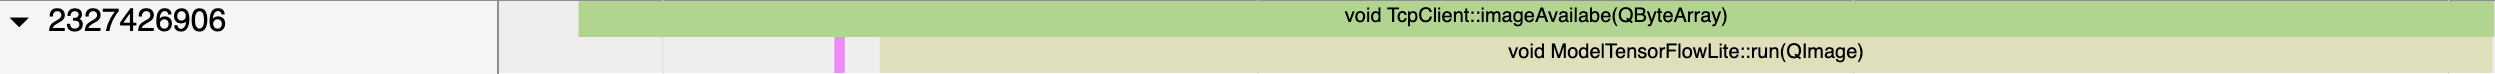
\includegraphics[width=\textwidth]{x86_64_1.jpg}} \\
	\subfloat[][\emph{time inference}.\label{subfig:time-inference}]%
		{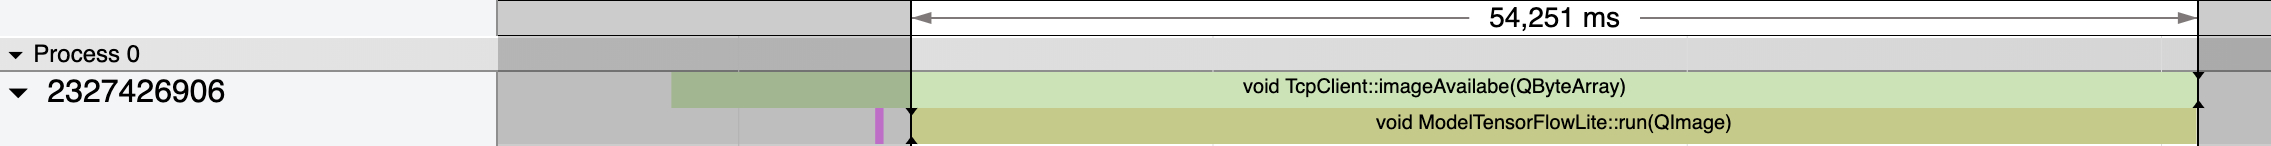
\includegraphics[width=\textwidth]{x86_64_2.jpg}} \\
	\subfloat[][\emph{total time cycle}.\label{subfig:time-cycle}]%
		{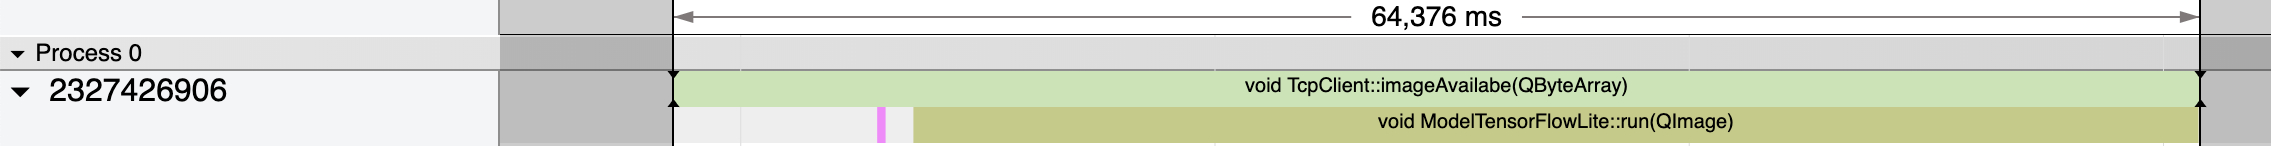
\includegraphics[width=\textwidth]{x86_64_3.jpg}}
	\caption{Visual benchmark inference on \texttt{x86\_64} architecture.}
	\label{fig:x86-bench}
\end{figure}
%
%
\subsection{Architecture armv7l}
\label{ssec:armv7l-bench-inference}